\section{Aufbau}
\label{sec:Aufbau}

\begin{figure}
\begin{minipage}{0.48\textwidth}
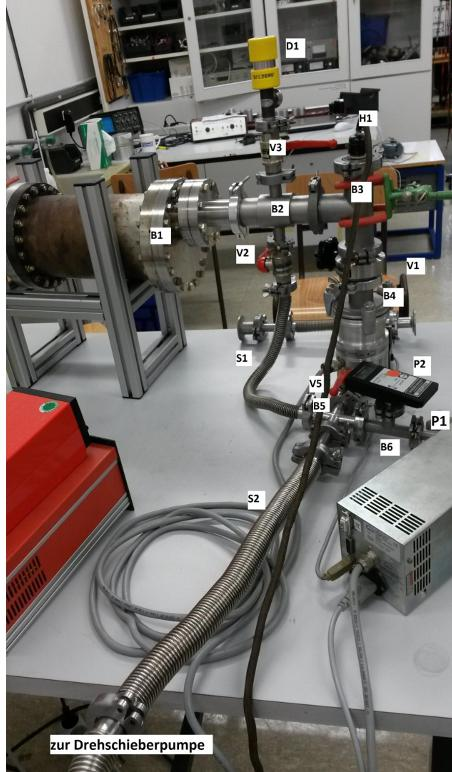
\includegraphics[scale=0.45]{content/images/Aufbau.jpg}
\caption{Aufbau zum Experiment Vakuumphysik\cite{V70}}
\label{fig:Aufbau}
\end{minipage}
\hfil
\begin{minipage}{0.42\textwidth}
Der Versuch wird wie in Abbildung \ref{fig:Aufbau} zu sehen aufgebaut. Dabei ist B1 der Rezipient.
\end{minipage}
\end{figure}